% Сборка: pdfLaTeX (Overleaf) или latexmk -pdf report.tex; картинки — в fig/.
\documentclass[11pt,a4paper]{article}
\usepackage[T2A]{fontenc}
\usepackage[utf8]{inputenc}
\usepackage[russian]{babel}
\usepackage[margin=2cm]{geometry}
\usepackage{amsmath}
\usepackage{graphicx}
\usepackage{booktabs}
\usepackage{caption}
\usepackage{enumitem}
\usepackage{textcomp}
\usepackage[hidelinks]{hyperref}

\graphicspath{{fig/}}
\captionsetup{font=small,labelsep=endash}
\setlist{nosep,leftmargin=*}
\newcommand{\todo}[1]{\textbf{[#1]}}

\title{Подбор геометрии подвески rocker-bogie\\ методом CMA-ES по динамическому моделированию}
\author{}
\date{}

\begin{document}
\maketitle

\begin{abstract}
Разработана программа, подбирающая геометрию рычагов шестиколёсной подвески rocker-bogie
под заданные габарит ($1200\times600$~мм), колесо и мотор. Каждый вариант геометрии
проверяется динамическими прогонами в физическом движке MuJoCo, а геометрия подбирается
эволюционной стратегией CMA-ES. Для мотор-колёс Xiaomi M365 Pro ($R=108$~мм, 16~Н$\cdot$м)
и массы ${\approx}\,50$~кг предел ступени вырос с 70~мм у исходной ручной геометрии
до ${\approx}\,500$~мм ($4{,}6R$; корпус в расчёте не участвует, см.~разд.~\ref{sec:limits}).
\end{abstract}

\section{Что считается проходимостью}

Ровер должен преодолевать одиночные препятствия передним и задним ходом.
Рассматриваются пять типовых препятствий по всей ширине хода (рис.~\ref{fig:obstacles}):
\begin{itemize}
  \item \textbf{подъём на ступень} высотой $h$ (вертикальная стенка);
  \item \textbf{съезд со ступени} высотой $h$;
  \item \textbf{ров} шириной $b$ и глубиной 500~мм. Глубина больше диаметра колеса,
        поэтому колесо не может опереться о дно, и ров проходится только перешагиванием;
  \item \textbf{кочка} --- блок высотой $h$ шириной 120~мм вдоль хода (кирпич плашмя)
        или 250~мм (небольшое бревно).
\end{itemize}
Кромки скруглены радиусом 10~мм: так учитывается обминание шины о кромку.

\begin{figure}[h]
  \centering
  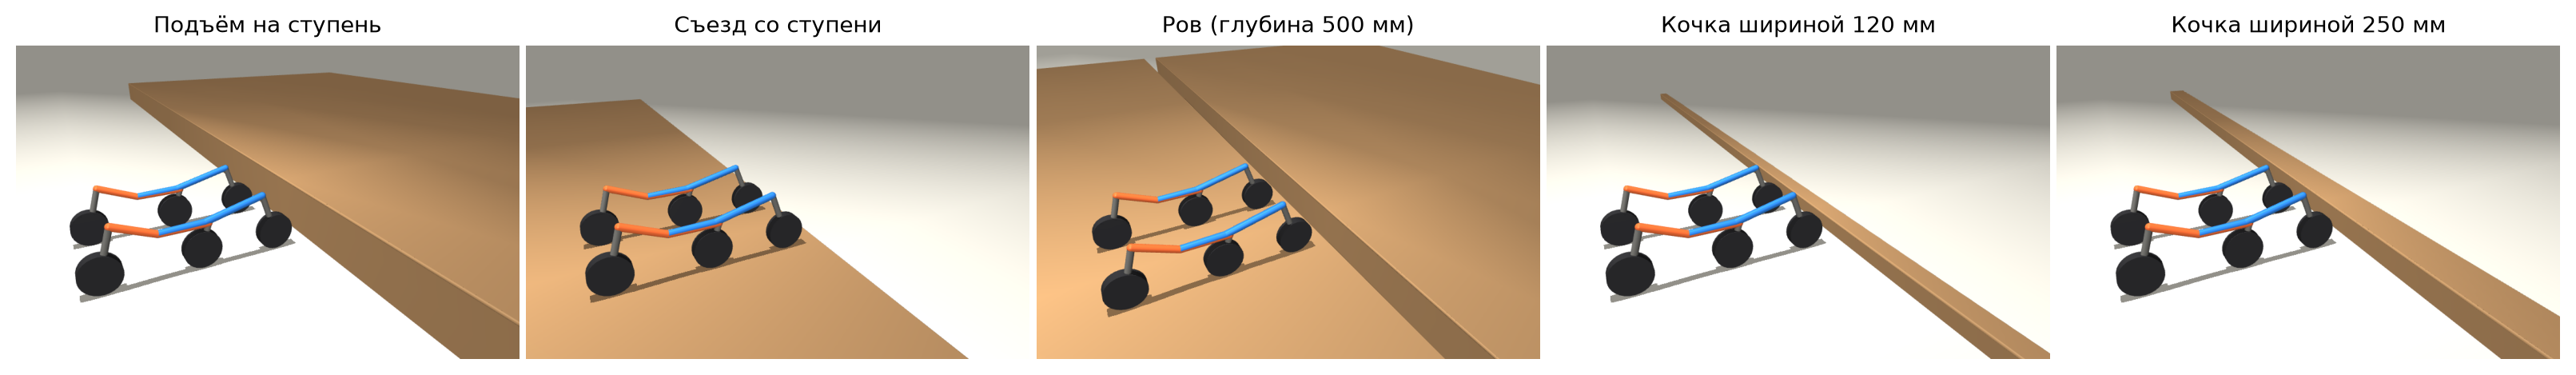
\includegraphics[width=\textwidth]{fig_obstacles.png}
  \caption{Типовые препятствия в MuJoCo (рендер). Рычаги rocker --- синие, bogie --- оранжевые}
  \label{fig:obstacles}
\end{figure}

Модель MuJoCo учитывает только то, что ограничивает проходимость:
\begin{itemize}
  \item \textbf{трение колёс} ($\mu=0{,}8$) --- предельная сила сцепления $f\le\mu N$,
        которой колесо цепляется за стенку и кромку;
  \item \textbf{пиковый момент мотора} --- предельная сила тяги колеса $\tau/R$;
        выше 4~м/с момент линейно падает до нуля на холостом ходу. Нагрев и КПД не учитываются;
  \item \textbf{упругая шина} --- обод подвешен к оси на пружине 100~Н/мм с демпфером.
        Без неё жёсткое колесо подпрыгивает на кромке, реакция опоры скачет от нуля до сотен
        ньютонов, и сцепление пропадает;
  \item \textbf{касания} труб рычагов и стоек о препятствие, \textbf{дифференциал} бортов
        и массы: корпус 25~кг, мотор-колёса $6\times4$~кг.
\end{itemize}

\textbf{Прогон успешен}, если все колёса оказались за препятствием. Он не засчитывается,
если рычаг или стойка задели препятствие, ровер опрокинулся либо завис:
колёса упёрлись и стоят на пиковом моменте или прокручиваются на месте.
Причина неудачи сохраняется. Она показывает, что ограничивает проходимость: геометрия, момент или сцепление.

\textbf{Проходимость по препятствию $i$} --- наибольший размер $h_i$ (высота, у рва --- ширина),
при котором прогон успешен. Он ищется бинарным поиском с точностью 5~мм, и каждая точка
поиска --- полный прогон.

Из двух направлений берётся \textbf{худшее}. Ровер может заехать туда, откуда выбраться
можно только задним ходом. Если назад он едет хуже, чем вперёд, он там застрянет, поэтому оба
направления считаются равноценными. Задание выраженного направления (как у автомобиля,
который вперёд едет лучше, чем назад) оставлено на будущее.

\section{Параметры и начальная точка}

Борт описан как плоский механизм (рис.~\ref{fig:params}). Каждый рычаг задаётся двумя плечами
и углом между ними, отсчитанным \emph{под шарниром}: при угле меньше $180^\circ$ шарнир выше
концов рычага (форма $\Lambda$), при угле больше $180^\circ$ --- ниже (форма V).
Такая запись всегда даёт собираемый рычаг, в отличие от координат шарниров.

\begin{figure}[h]
  \centering
  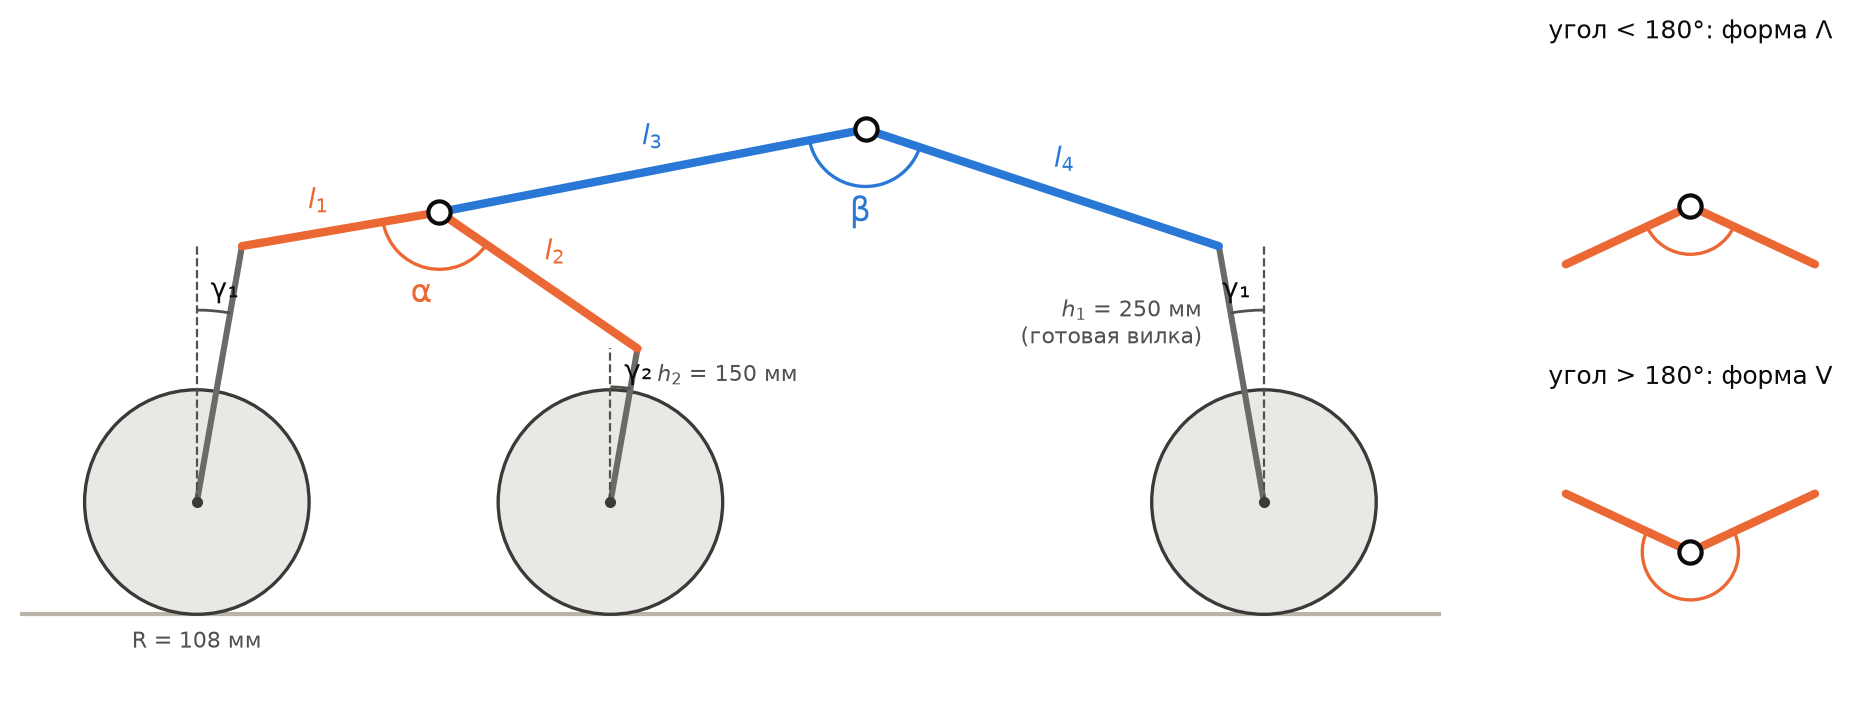
\includegraphics[width=\textwidth]{fig_params.png}
  \caption{Параметры борта. Оптимизируются плечи $l_1$--$l_4$, углы рычагов $\alpha$, $\beta$
  и наклоны стоек $\gamma_1$, $\gamma_2$. Высоты стоек $h_1$, $h_2$ и радиус колеса $R$ фиксированы.
  Справа --- формы рычага в зависимости от угла}
  \label{fig:params}
\end{figure}

Оптимизируются восемь параметров:
\begin{itemize}
  \item bogie: плечи $l_1$, $l_2$ (100--450~мм) и угол $\alpha$ (100--$280^\circ$);
  \item rocker: плечи $l_3$ (150--600~мм), $l_4$ (200--750~мм) и угол $\beta$ (100--$280^\circ$);
  \item наклоны стоек: крайних колёс $\gamma_1$ (зеркально спереди и сзади)
        и среднего колеса $\gamma_2$ (оба $\pm25^\circ$).
\end{itemize}

\textbf{Фиксированы} размеры покупных узлов: высота стоек крайних колёс $h_1=250$~мм
(готовая вилка M365 Pro с рулевой колонкой), высота стойки среднего колеса $h_2=150$~мм,
радиус колеса $R=108$~мм, а также масса и момент.

\textbf{Недопустимой} считается геометрия, которую нельзя собрать или которая не влезает
в габарит. Такая геометрия не моделируется:
\begin{itemize}
  \item длина больше 1200~мм;
  \item шарниры ниже диаметра колеса;
  \item соседние колёса пересекаются;
  \item шарнир bogie не между задним и средним колёсами или главный шарнир не между средним и передним;
  \item плечи не дотягиваются до стоек.
\end{itemize}

\textbf{Начальная точка} --- геометрия, введённая вручную по изображениям марсоходов:
колёса в точках 0, 380 и 940~мм, главный шарнир $(600;\,470)$~мм, шарнир bogie
$(190;\,390)$~мм, стойки вертикальны. Это $l_1/l_2=193/231$~мм, $\alpha=136^\circ$,
$l_3/l_4=418/358$~мм, $\beta=151^\circ$: оба рычага $\Lambda$-образные
(рис.~\ref{fig:designs}, слева). Такая геометрия проходит ступень всего 70~мм.

\section{Метрика}

Оптимизатор сравнивает варианты только по одному числу, поэтому пять пределов $h_i$
сводятся в оценку
\begin{equation}
  J=\sum_i w_i h_i \;\to\; \max,\qquad
  w_{\text{ступень}}=1,\; w_{\text{съезд}}=0{,}3,\; w_{\text{ров}}=w_{\text{кочки}}=0{,}5 .
  \label{eq:J}
\end{equation}
$J$ --- взвешенная сумма пределов в миллиметрах. Каждый миллиметр прироста предела
добавляет к оценке свой вес, так что вес задаёт <<цену>> препятствия: оптимизатор согласится
уменьшить кочку на 10~мм, только если ступень вырастет больше чем на 5~мм.
\begin{itemize}
  \item \textbf{Ступень} --- самое трудное и характерное для rocker-bogie препятствие,
        поэтому у неё наибольший вес.
  \item \textbf{Съезд} считается проще подъёма, и пределы у него большие; малый вес не даёт
        ему заглушить остальные слагаемые.
  \item \textbf{Кочки} проверяют то, чего не видит ступень: узкое препятствие проходит между
        колёсами и может задеть трубу рычага.
\end{itemize}
Влияние весов на итоговую геометрию разобрано в разд.~\ref{sec:weights}.

В программе есть и вторая цель --- \textbf{наименьший момент колеса}, при котором проходится
заданный набор препятствий. Колесо лезет по стенке только за счёт трения, а оно ограничено
моментом ($f\le\tau/R$). Поэтому момент --- физический ограничитель, и он меняется с геометрией
плавно. Однако если хоть одно препятствие непроходимо при любом моменте, цель становится
бесконечной у большинства вариантов. Поэтому основной выбрана $J$.

\section{Метод оптимизации}

Градиент у $J$ бесполезен:
\begin{itemize}
  \item исход прогона двоичный, а предел округлён до шага поиска, так что при малом изменении
        геометрии $J$ либо не меняется, либо прыгает скачком;
  \item взятие худшего направления даёт изломы;
  \item касание, отрыв и проскальзывание колёс переключаются скачком.
\end{itemize}
Поэтому применена безградиентная эволюционная стратегия \textbf{CMA-ES}
(Covariance Matrix Adaptation Evolution Strategy, библиотека \texttt{cma}).

Метод хранит не один вариант, а облако вариантов --- многомерное нормальное распределение
со средним $m$, ковариацией $C$ и шагом $\sigma$. Каждое поколение устроено так:
\begin{enumerate}
  \item из распределения выбирается $\lambda=10$ новых геометрий;
  \item каждая оценивается по~(\ref{eq:J}) --- это и есть дорогие прогоны MuJoCo;
  \item среднее $m$ сдвигается к взвешенному центру лучшей половины, т.\,е. к удачным геометриям;
  \item матрица $C$ вытягивается вдоль направлений, в которых были сделаны удачные шаги.
        Например, если помогает одновременно удлинить плечо и уменьшить угол, облако вытянется
        вдоль этой связки;
  \item шаг $\sigma$ растёт, пока шаги идут в одну сторону, и уменьшается, когда поиск
        топчется на месте.
\end{enumerate}

Каждая геометрия оценивается заново по всем препятствиям. Метод не <<доучивает>> найденный
вариант на новых препятствиях, а значит, и <<забыть>>, как проходить мелкие препятствия, не может.

Детали реализации:
\begin{enumerate}
  \item Параметры нормируются в $[0,1]$. Старт --- начальная геометрия, $\sigma_0=0{,}3$.
  \item Недопустимая геометрия не моделируется и получает штраф $10^4$ плюс величина нарушения
        в миллиметрах. Так метод видит, в какую сторону возвращаться в допустимую область.
  \item Поиск каждого предела начинается от значения у лучшего на данный момент варианта:
        это в 1,5--2 раза сокращает число прогонов.
\end{enumerate}
Все пары <<вариант $\times$ препятствие $\times$ направление>> поколения считаются параллельно.
20 поколений --- это 200 геометрий, или около 2000 поисков пределов, и занимают ${\approx}\,15$~мин
на 16 ядрах.

\section{Результаты}

\subsection{Сходимость и начальная точка}

На рис.~\ref{fig:cmaes} --- запуск из начальной геометрии: за 7 поколений $J$ выросла
с 304 до ${\approx}\,550$~мм. Облако вариантов (точки) при этом не сжимается к лучшему: медиана поколения
колеблется около 300--400~мм. Причина --- кусочно-постоянная $J$. Шаг поиска предела 5~мм,
и исход прогона двоичный, поэтому у лучшей точки почти все соседи имеют ту же или меньшую
оценку, а улучшение возможно только скачком через <<порог>> --- например, когда труба
перестаёт задевать кромку. Метод долго не находит такой скачок и останавливается на плато,
т.\,е. в локальном максимуме.

Чтобы оценить, насколько результат зависит от старта, запуск повторён с той же ручной
геометрией и другими случайными выборками (seed), из варианта (3) и из двух случайных
допустимых геометрий (рис.~\ref{fig:starts}). Все запуски --- по 20 поколений с одинаковой
метрикой. Итоговая $J$ разбросана от 481 до 877~мм, и даже один и тот же старт с разным seed
даёт 555, 729 и 801~мм. Вариант (3), полученный ранее более длинными запусками, за 20 поколений
улучшить не удалось: он оказался лучшим из найденных максимумов.

Вывод: начальная точка и случайность заметно влияют на результат, и метод находит локальные,
а не глобальный максимум. На практике оптимизацию нужно запускать несколько раз (из разных
точек или с разным seed) и брать лучший результат, а найденный вариант дополнительно
перезапускать как новую начальную точку. Именно так получен вариант (3).

\begin{figure}[h]
  \centering
  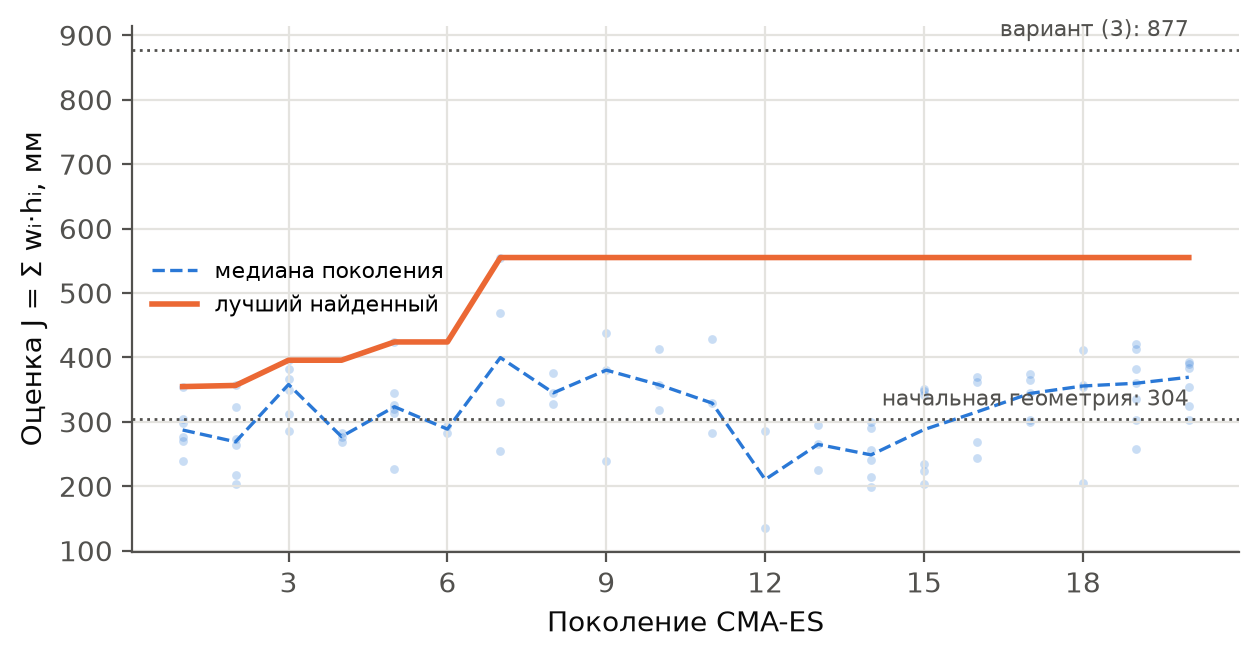
\includegraphics[width=0.75\textwidth]{fig_cmaes.png}
  \caption{Запуск CMA-ES из начальной геометрии: точки --- варианты поколения, пунктир ---
  медиана поколения, линия --- лучший найденный вариант. Пунктирные уровни --- начальная
  геометрия и вариант (3)}
  \label{fig:cmaes}
\end{figure}

\begin{figure}[h]
  \centering
  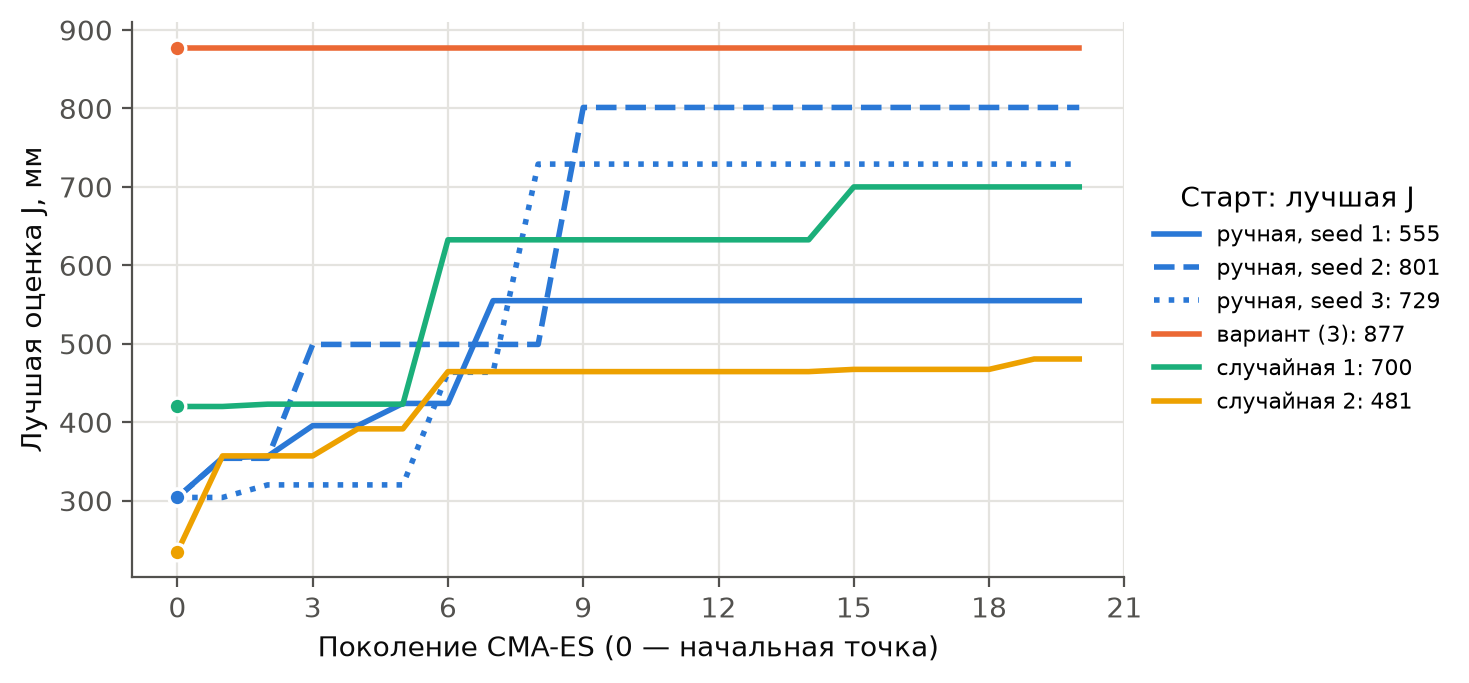
\includegraphics[width=0.85\textwidth]{fig_starts.png}
  \caption{Лучшая $J$ по поколениям из разных начальных точек и с разными seed}
  \label{fig:starts}
\end{figure}

Пределы найденных геометрий (худшее направление, мм; $J$ --- с базовыми весами):

\begin{center}
\begin{tabular}{lcccccc}
\toprule
Геометрия & ступень & съезд & ров & кочка 120 & кочка 250 & $J$ \\
\midrule
Начальная (ручная) & 70 & 239 & 184 & 70 & 70 & 304 \\
Ручная, seed 1 & 197 & 427 & 188 & 131 & 131 & 550 \\
Ручная, seed 2 & 422 & 394 & 207 & 122 & 202 & 805 \\
Вариант (3) & 502 & 525 & 207 & 127 & 103 & 877 \\
\midrule
Упор на ступень & 104 & 427 & 184 & 104 & 104 & 427 \\
Упор на кочки & 108 & 427 & 191 & 127 & 286$^*$ & 538 \\
Равные веса & 84 & 384 & 188 & 150 & 272 & 504 \\
\bottomrule
\end{tabular}
\end{center}
{\small $^*$ кочку 110~мм эта геометрия не проходит, см.~разд.~\ref{sec:trap}.}

$J$ --- это сумма по всем препятствиям, поэтому её рост не означает роста каждого предела.
Например, у запуска <<ручная, seed 1>> ступень всего 197~мм. Причина --- худшее направление:
задним ходом эта геометрия берёт 520~мм, а передним только 200~мм (рис.~\ref{fig:heights}).

\begin{figure}[h]
  \centering
  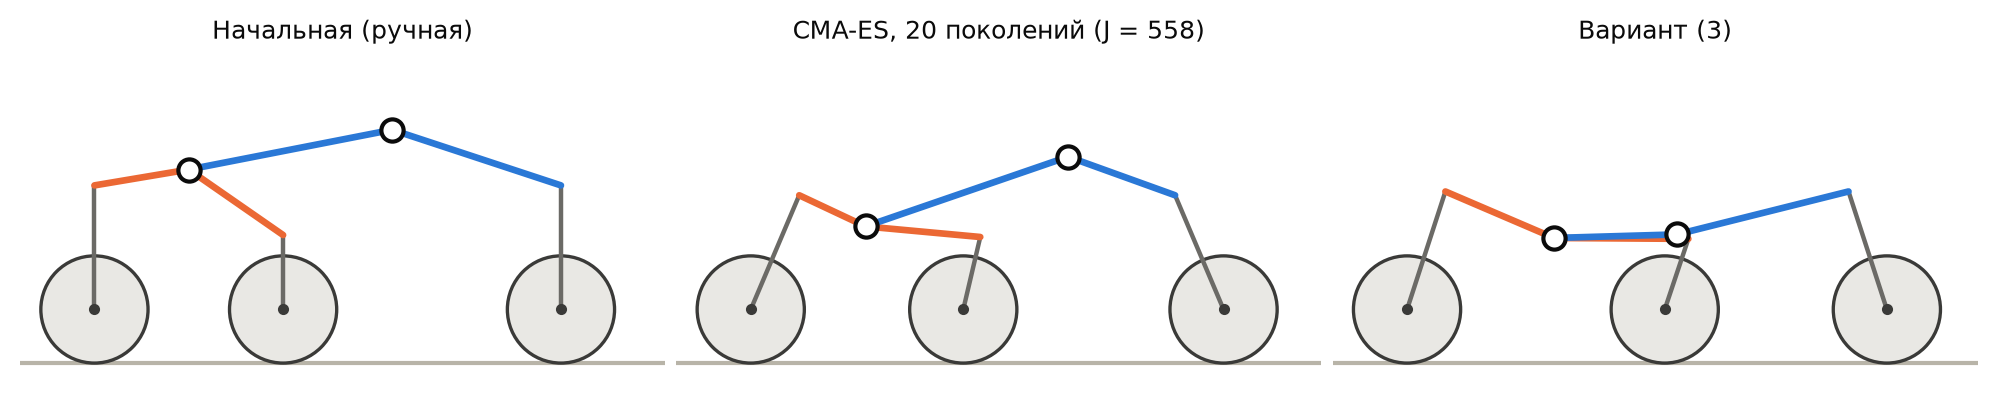
\includegraphics[width=\textwidth]{fig_designs.png}
  \caption{Начальная геометрия, результат 20 поколений CMA-ES и вариант (3) в одном масштабе}
  \label{fig:designs}
\end{figure}

\subsection{Влияние весов метрики}
\label{sec:weights}

Из той же ручной геометрии с тем же seed запущены три набора весов
(ступень / съезд / ров / кочки):
\begin{itemize}
  \item <<упор на ступень>>: 1 / 0,1 / 0,1 / 0,1;
  \item <<упор на кочки>>: 0,3 / 0,1 / 0,3 / 1;
  \item <<равные веса>>: все по 1.
\end{itemize}
Геометрии показаны на рис.~\ref{fig:weights}, пределы --- в таблице выше.

Веса заметно меняют то, на что работает геометрия. При упоре на кочки и равных весах кочка
250~мм выросла до 272--286~мм (у остальных запусков 103--202~мм), но ступень упала до 84--108~мм.
Rocker при упоре на кочки стал сильно $\Lambda$-образным ($\beta=118^\circ$) и высоко поднял
главный шарнир. При равных весах два параметра ушли на границы диапазона ($l_1=101$~мм,
$l_4=200$~мм), т.\,е. оптимизатору <<не хватило>> диапазона.

Упор на ступень, напротив, дал ступень всего 104~мм, хуже базовых весов. Причина та же, что
в предыдущем разделе: запуск застрял в локальном максимуме, и разброс между seed (550--805~мм)
больше, чем эффект весов. По одному запуску на набор весов можно судить о направлении, куда
сдвигается геометрия, но не о величине эффекта: для этого нужно по нескольку запусков на набор.

\begin{figure}[h]
  \centering
  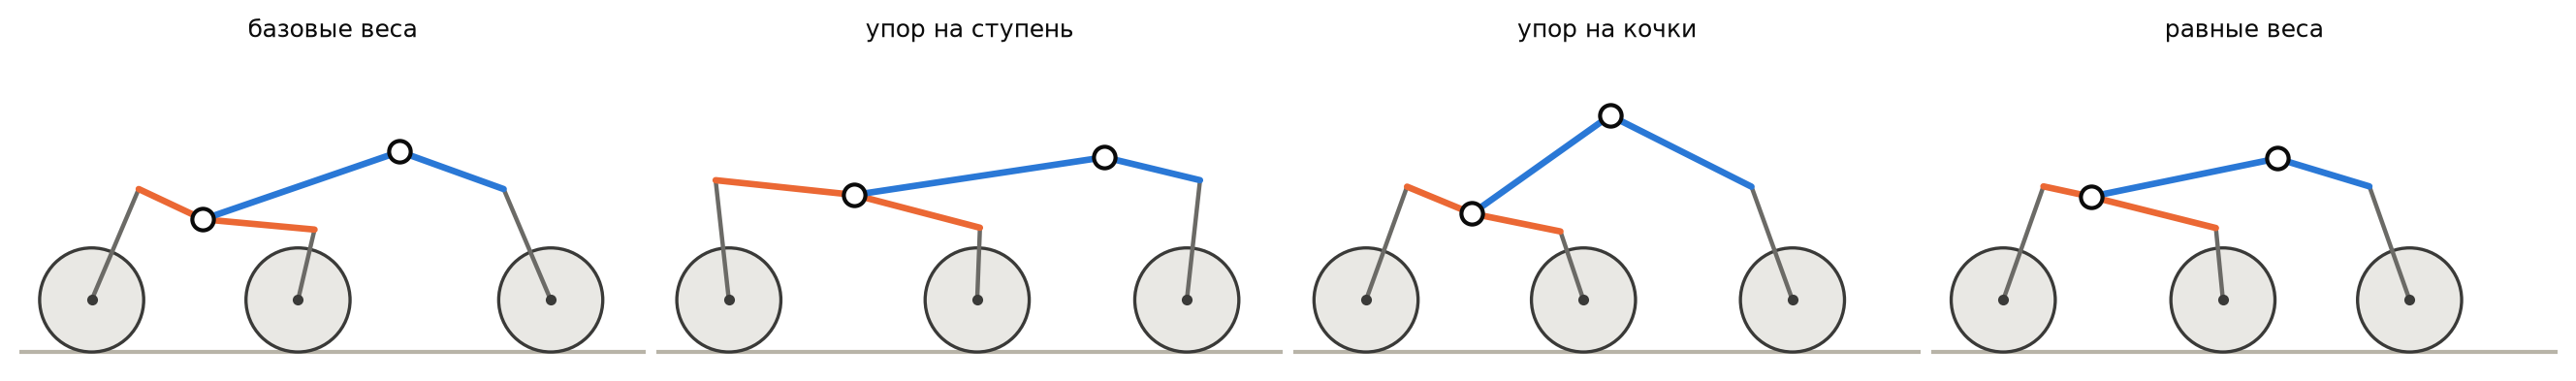
\includegraphics[width=\textwidth]{fig_weights_designs.png}
  \caption{Геометрии, найденные при разных весах метрики (один старт и seed)}
  \label{fig:weights}
\end{figure}

\subsection{Посадка на мель}
\label{sec:trap}

Бинарный поиск предполагает, что всё ниже найденного предела тоже проходится. Если геометрия
садится на мель на невысоком препятствии и при этом проходит высокое, поиск этого не заметит.
Поэтому найденные геометрии проверены на всех размерах препятствий с шагом 10~мм
(рис.~\ref{fig:heights}).

У варианта (3) и у запусков с базовыми весами непроходимых размеров ниже предела нет:
проходимые высоты идут сплошной полосой от нуля. Отдельные <<островки>> встречаются только
у съезда вблизи предела. Например, вариант (3) не съезжает с 490--500~мм, но съезжает
с 510--560~мм.

Геометрия, найденная при \textbf{упоре на кочки}, на мель садится. Кочку шириной 250~мм
передним ходом она проходит до 100~мм, на 110~мм застревает (не хватает момента), а затем
снова проходит 120--280~мм. Задним ходом она застревает на 230~мм и снова проходит 240--280~мм. Бинарный поиск этой дыры
не заметил и записал предел 286~мм, и оптимизатор выбрал геометрию за большую <<высоту
кочки>>. В реальности такой ровер проедет бревно высотой 250~мм, но встанет перед бревном
110~мм.

Это пример геометрии, которая выглядит лучше по метрике, но не работает. Чтобы оптимизатор
её отбраковывал, предел нужно считать <<сплошным>>: проверять все размеры снизу вверх с
шагом 10--20~мм до первой неудачи. Это в 2--3 раза дороже бинарного поиска, поэтому
разумно применять такую проверку к лучшим вариантам перед выдачей результата.

\begin{figure}[h]
  \centering
  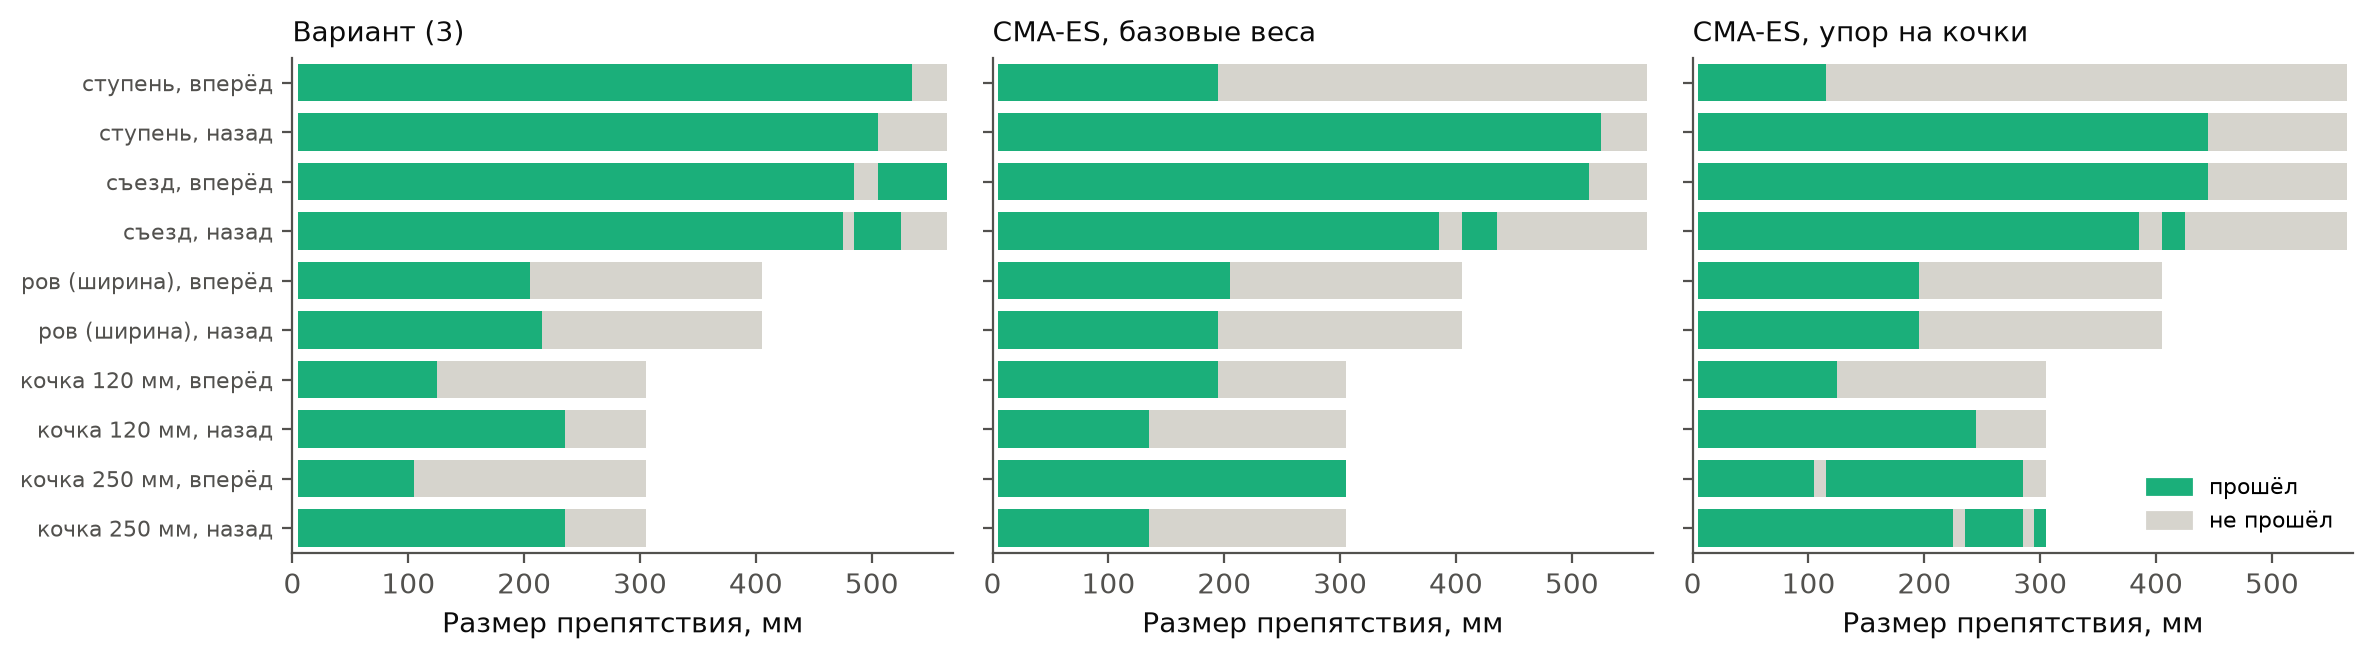
\includegraphics[width=\textwidth]{fig_heights.png}
  \caption{Прогоны на всех размерах препятствий с шагом 10~мм. Справа --- геометрия,
  найденная при упоре на кочки: дыра на кочке 250~мм при высоте 110~мм}
  \label{fig:heights}
\end{figure}

\subsection{Момент мотора и закон управления}

Каждая точка на рис.~\ref{fig:torque} и~\ref{fig:radius} --- медиана по трём скоростям
подъезда (0,12/0,15/0,18~м/с), полоса --- разброс между ними.

У начальной геометрии предел ${\approx}\,70$~мм не растёт с моментом. Передним ходом задние
колёса при малом моменте упираются, а при большом пробуксовывают: геометрия не прижимает их
к кромке, т.\,е. ограничение геометрическое. У варианта (3) до 10~Н$\cdot$м предел
ограничен моментом (56--112~мм), а с 12~Н$\cdot$м выходит на ${\approx}\,500$~мм. Там его
ограничивают касание трубы bogie и сцепление.

Провал на 11--14~Н$\cdot$м --- это порог: момента хватает впритык, и малое изменение скорости
меняет последовательность контактов. При 13~Н$\cdot$м предел составил 499, 316 и 436~мм
при трёх скоростях. Сеточный прогон показал, что при 13~Н$\cdot$м не проходятся только ступени
320--340~мм, а 360--520~мм проходятся. Бинарный поиск попадает в такую <<дырку>>
и даёт заниженный предел. Вдали от порога разброса нет.

Колёсами можно управлять двумя способами:
\begin{itemize}
  \item \textbf{регулятор скорости на каждом колесе}: колесо держит заданную скорость,
        пока хватает пикового момента;
  \item \textbf{одинаковый момент всех колёс}, задаваемый регулятором скорости корпуса.
\end{itemize}
Регулятор скорости на колесе не прибавляет момент, пока колесо крутится с заданной скоростью.
Пробуксовка в нём означает, что колесо крутится, а сила трения о стенку не поднимает ровер.

Закон управления заметно влияет на результат. При одинаковом моменте 25--40~Н$\cdot$м предел
варианта (3) зависит от скорости подъезда: от 352 до 506~мм (пунктир на рис.~\ref{fig:torque}).
При регуляторах скорости он устойчиво равен 499~мм. На увеличенных колёсах картина обратная
(рис.~\ref{fig:radius}): при регуляторах скорости и 24~Н$\cdot$м колёса с $R\ge130$~мм
пробуксовывают на стенке, а при одинаковом моменте предел растёт до 820~мм.
Вывод: геометрию нужно подбирать под тот закон управления, который будет стоять на ровере.
Вариант (3) подобран под регуляторы скорости.

\begin{figure}[h]
  \centering
  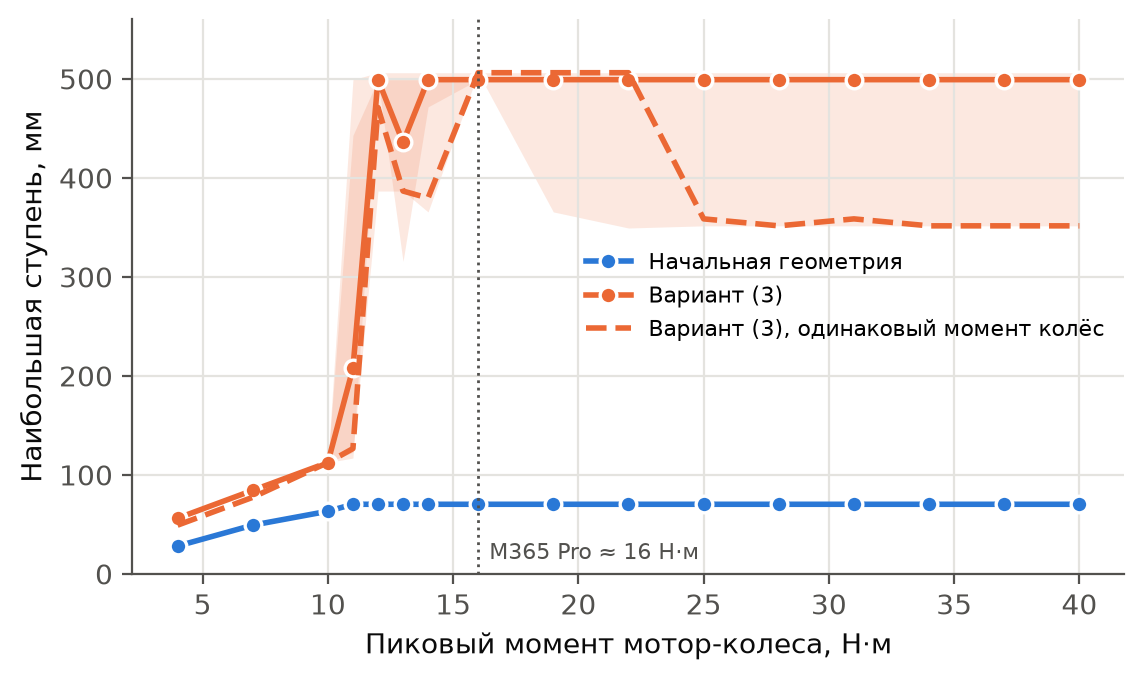
\includegraphics[width=0.75\textwidth]{fig_torque.png}
  \caption{Наибольшая ступень в зависимости от пикового момента колеса (худшее направление)}
  \label{fig:torque}
\end{figure}

\subsection{Радиус колеса}

Чтобы не привязываться к конкретному колесу, вариант (3) масштабировался подобно (все длины
$\propto R$) при неизменной массе (рис.~\ref{fig:radius}). Видны три режима:
\begin{itemize}
  \item \textbf{геометрический}: пока хватает момента, предел растёт линейно, $h\approx4$--$4{,}7R$,
        т.\,е. вдвое больше диаметра колеса;
  \item \textbf{моментный}: требуемый момент $\tau\approx F R$ растёт с радиусом. Поэтому при
        16~Н$\cdot$м и $R\ge160$~мм предел обрушивается до ${\approx}\,170$~мм, а при 8~Н$\cdot$м
        он ${\approx}\,90$~мм при любом радиусе;
  \item \textbf{сцепной}: колёса пробуксовывают на стенке (24~Н$\cdot$м, регуляторы скорости).
\end{itemize}
Колесо выгодно увеличивать, только если момент растёт вместе с радиусом.

\begin{figure}[h]
  \centering
  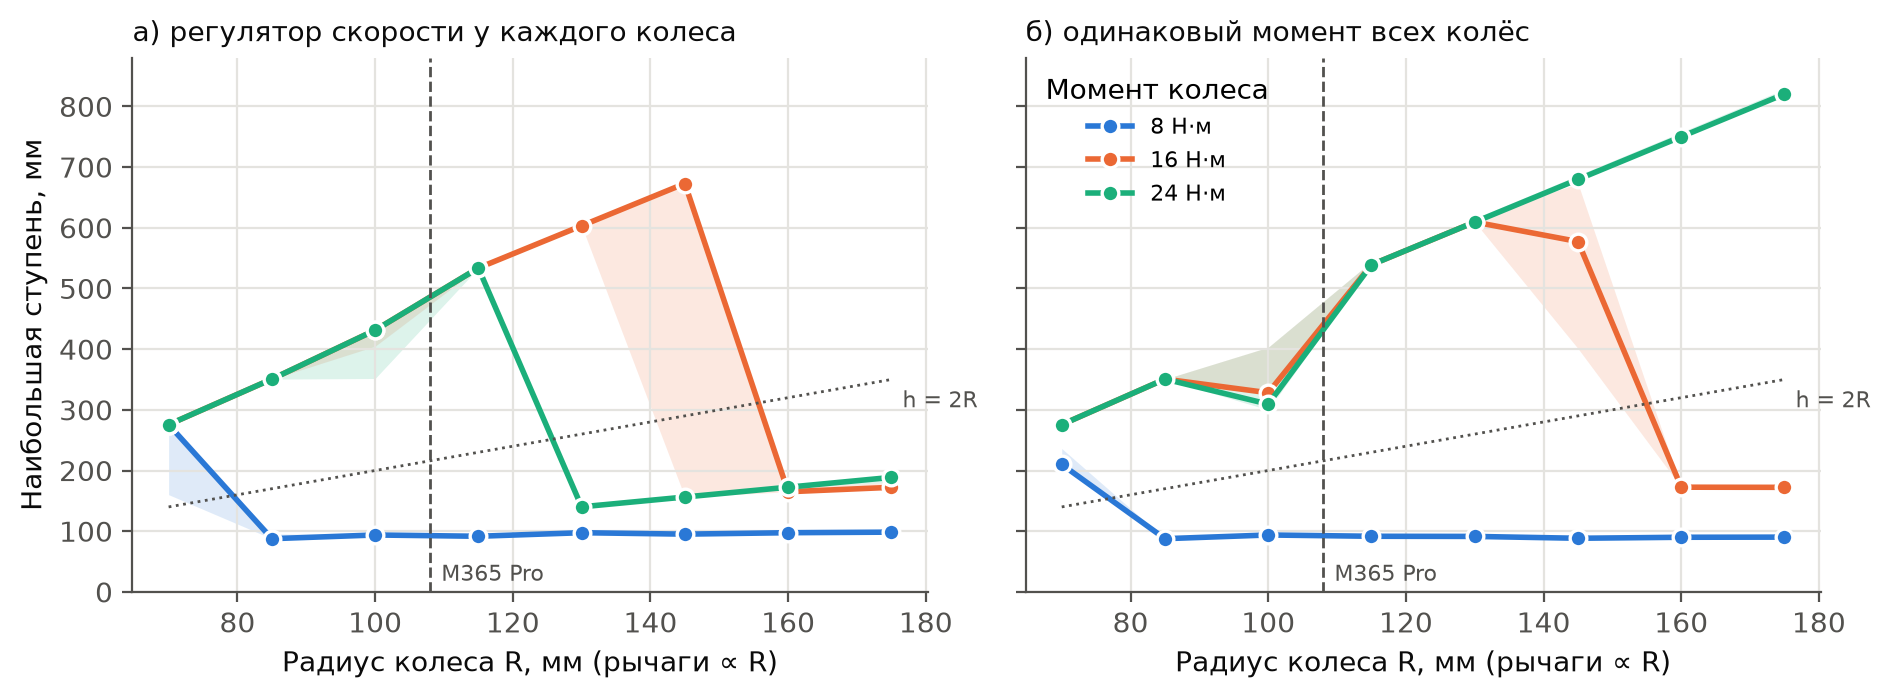
\includegraphics[width=\textwidth]{fig_radius.png}
  \caption{Наибольшая ступень в зависимости от радиуса колеса при подобном масштабировании
  рычагов: а)~регулятор скорости на каждом колесе; б)~одинаковый момент всех колёс}
  \label{fig:radius}
\end{figure}

\subsection{Форма рычагов}

На рис.~\ref{fig:geometry} у варианта (3) меняются только углы $\alpha$ и $\beta$. Изменение угла
на $10^\circ$ меняет предел не плавно, а скачком: например, при $\beta=190^\circ$ переход
$\alpha$ с 190 на $200^\circ$ поднимает предел со 120 до 499~мм. За таким скачком стоит смена
механизма отказа: при одном угле труба задевает кромку или колесо упирается, при соседнем
--- нет.

Высокий предел (470--510~мм) даёт только узкая область: слегка V-образный bogie
($\alpha=190$--$210^\circ$) и rocker с $\beta=160$--$190^\circ$. $\Lambda$-образный bogie даёт
не более 180~мм. Штриховкой отмечена недопустимая геометрия.

\begin{figure}[h]
  \centering
  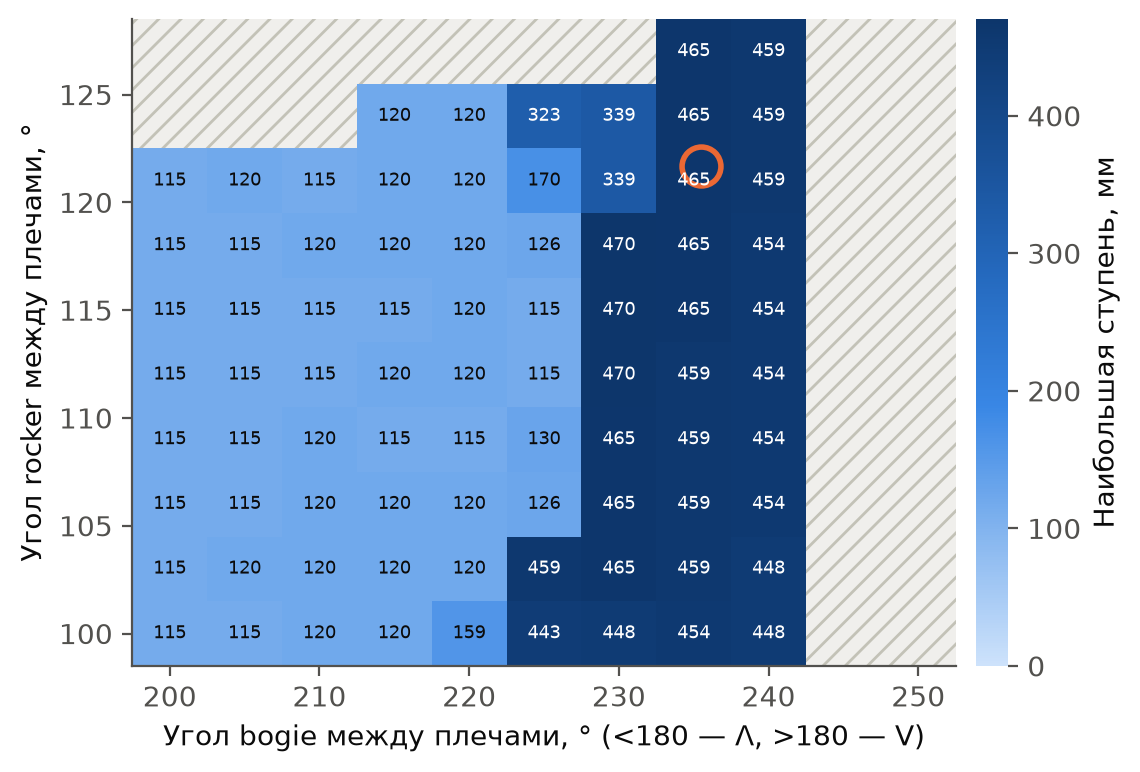
\includegraphics[width=0.7\textwidth]{fig_geometry.png}
  \caption{Наибольшая ступень при 16~Н$\cdot$м в зависимости от углов bogie и rocker
  (остальные параметры --- как у варианта (3), отмечен кружком)}
  \label{fig:geometry}
\end{figure}

\subsection{Пример прохождения}

На рис.~\ref{fig:climb} вариант (3) поднимается на ступень 500~мм. Анимация ---
файл \texttt{fig/step\_500.gif}.

\begin{figure}[h]
  \centering
  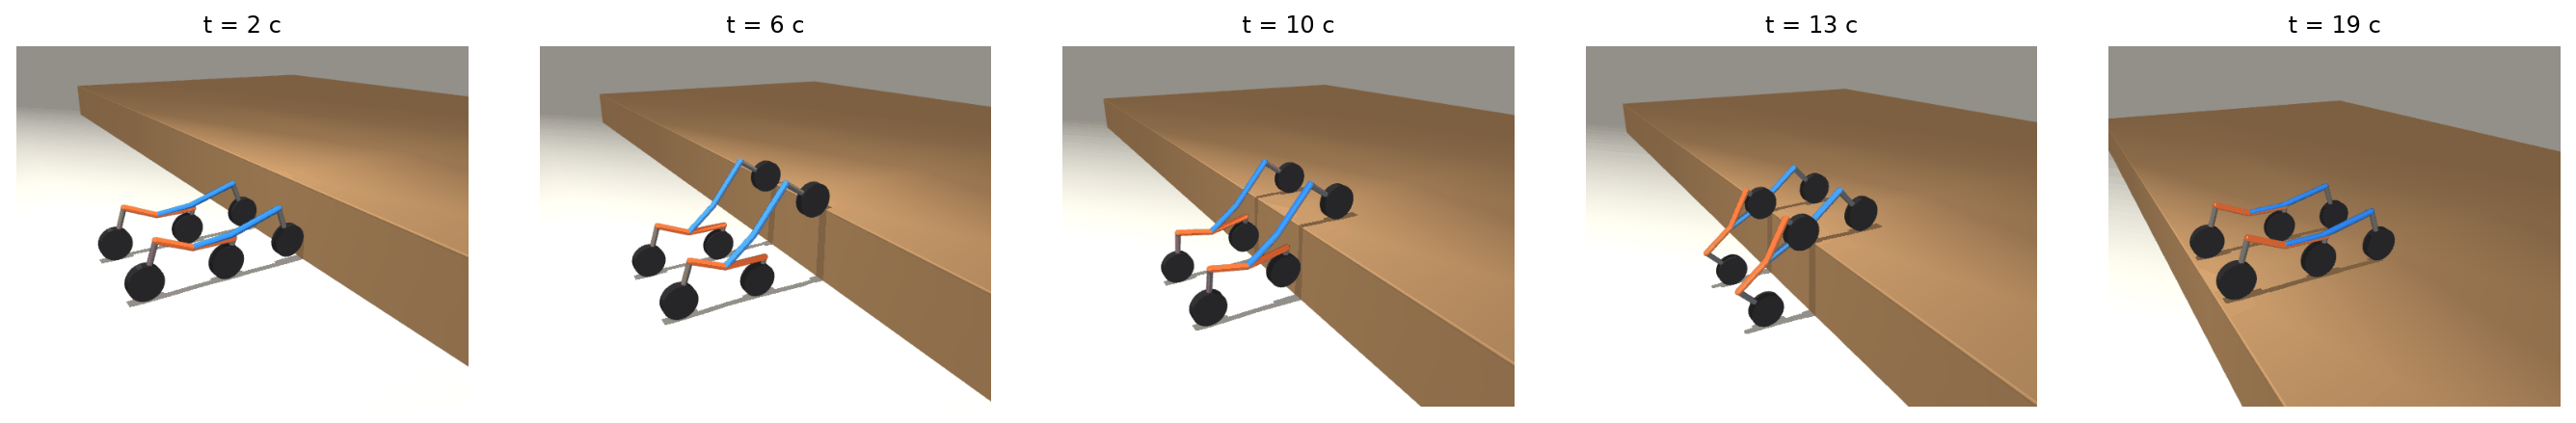
\includegraphics[width=\textwidth]{fig_climb.png}
  \caption{Подъём варианта (3) на ступень 500~мм (кадры MuJoCo; корпус не показан, т.\,к.\ в расчёте не участвует)}
  \label{fig:climb}
\end{figure}

\section{Ограничения модели}
\label{sec:limits}

\begin{itemize}
  \item \textbf{Корпус в столкновениях не участвует.} Его размеры зависят от полезной нагрузки
        и пока не заданы. На ступени 300~мм условный корпус (ящик высотой 100~мм над главными
        шарнирами) заходит в препятствие на 26~мм, на 500~мм --- на 165~мм. Поэтому пределы выше
        ${\approx}\,250$~мм относятся к подвеске без корпуса; реальный корпус их уменьшит.
  \item \textbf{Рычаги не проверяются на взаимное пересечение.} У варианта (3) переднее плечо
        bogie почти совпадает с задним плечом rocker, поэтому в конструкции bogie нужно разнести
        с rocker по ширине.
  \item Грунт жёсткий, препятствия --- по всей ширине хода, колёса не поворачиваются.
\end{itemize}

\section{Выводы}
\todo{выводы перепишем позже}

\section{Дальнейшая работа}
\begin{itemize}
  \item Ввести в метрику \textbf{экономичность}: момент колеса, взвешенный по вероятности
        препятствия. Мелкие препятствия встречаются чаще, и их нужно проходить экономно,
        а крупные --- хотя бы проходить. Это минимизация средней ожидаемой энергии прохождения.
  \item Задавать \textbf{выраженное направление} движения: разные веса для переднего и заднего хода.
  \item Добавить \textbf{корпус} в столкновения, когда будут известны его размеры.
\end{itemize}

\end{document}
